
%we experiment with the dataset proposed by \cite{luo2016temporal} which aims at extracting relations between entity and time. With some heuristics, this dataset can be further split intro three subsets with different levels of reliability, which enables us to conduct all our experiment settings. To show the generalization ability of our model, we also experiment with the dataset proposed by \cite{riedel2010modeling}, which aims at extracting relations between entities and there is no prior knowledge of the data quality can be used. \todo{can be shorter}

%We also consider two types of relation extraction tasks. The first task aims at extracting relations between entity and time. Specifically, it requires the object to be an time expression and the subject to be an entity. As suggested by \cite{luo2016temporal}, the distant supervision dataset in this task can be naturally divided into several subsets with different levels of reliability. The basic idea is that number of important things related to one entity increases as the time scope becomes larger. For example, a sentence containing both \emph{Alphabet} and \emph{October\_2\_2015} is very likely to express the foundation time of \emph{Alphabet}, while a sentence containing both \emph{Alphabet} and \emph{2015} may instead talk about its financial report of year 2015. We experiment with this task because it has a public dataset that contains both reliable and unreliable data, which enables us to conduct all of our experiments.

%The second task aims at extracting relations between entities, which is extensively studied in relation extraction. We experiment with this task to see if our transition matrix method generalizes well in different datasets.

\begin{figure}[t!]
\begin{center}
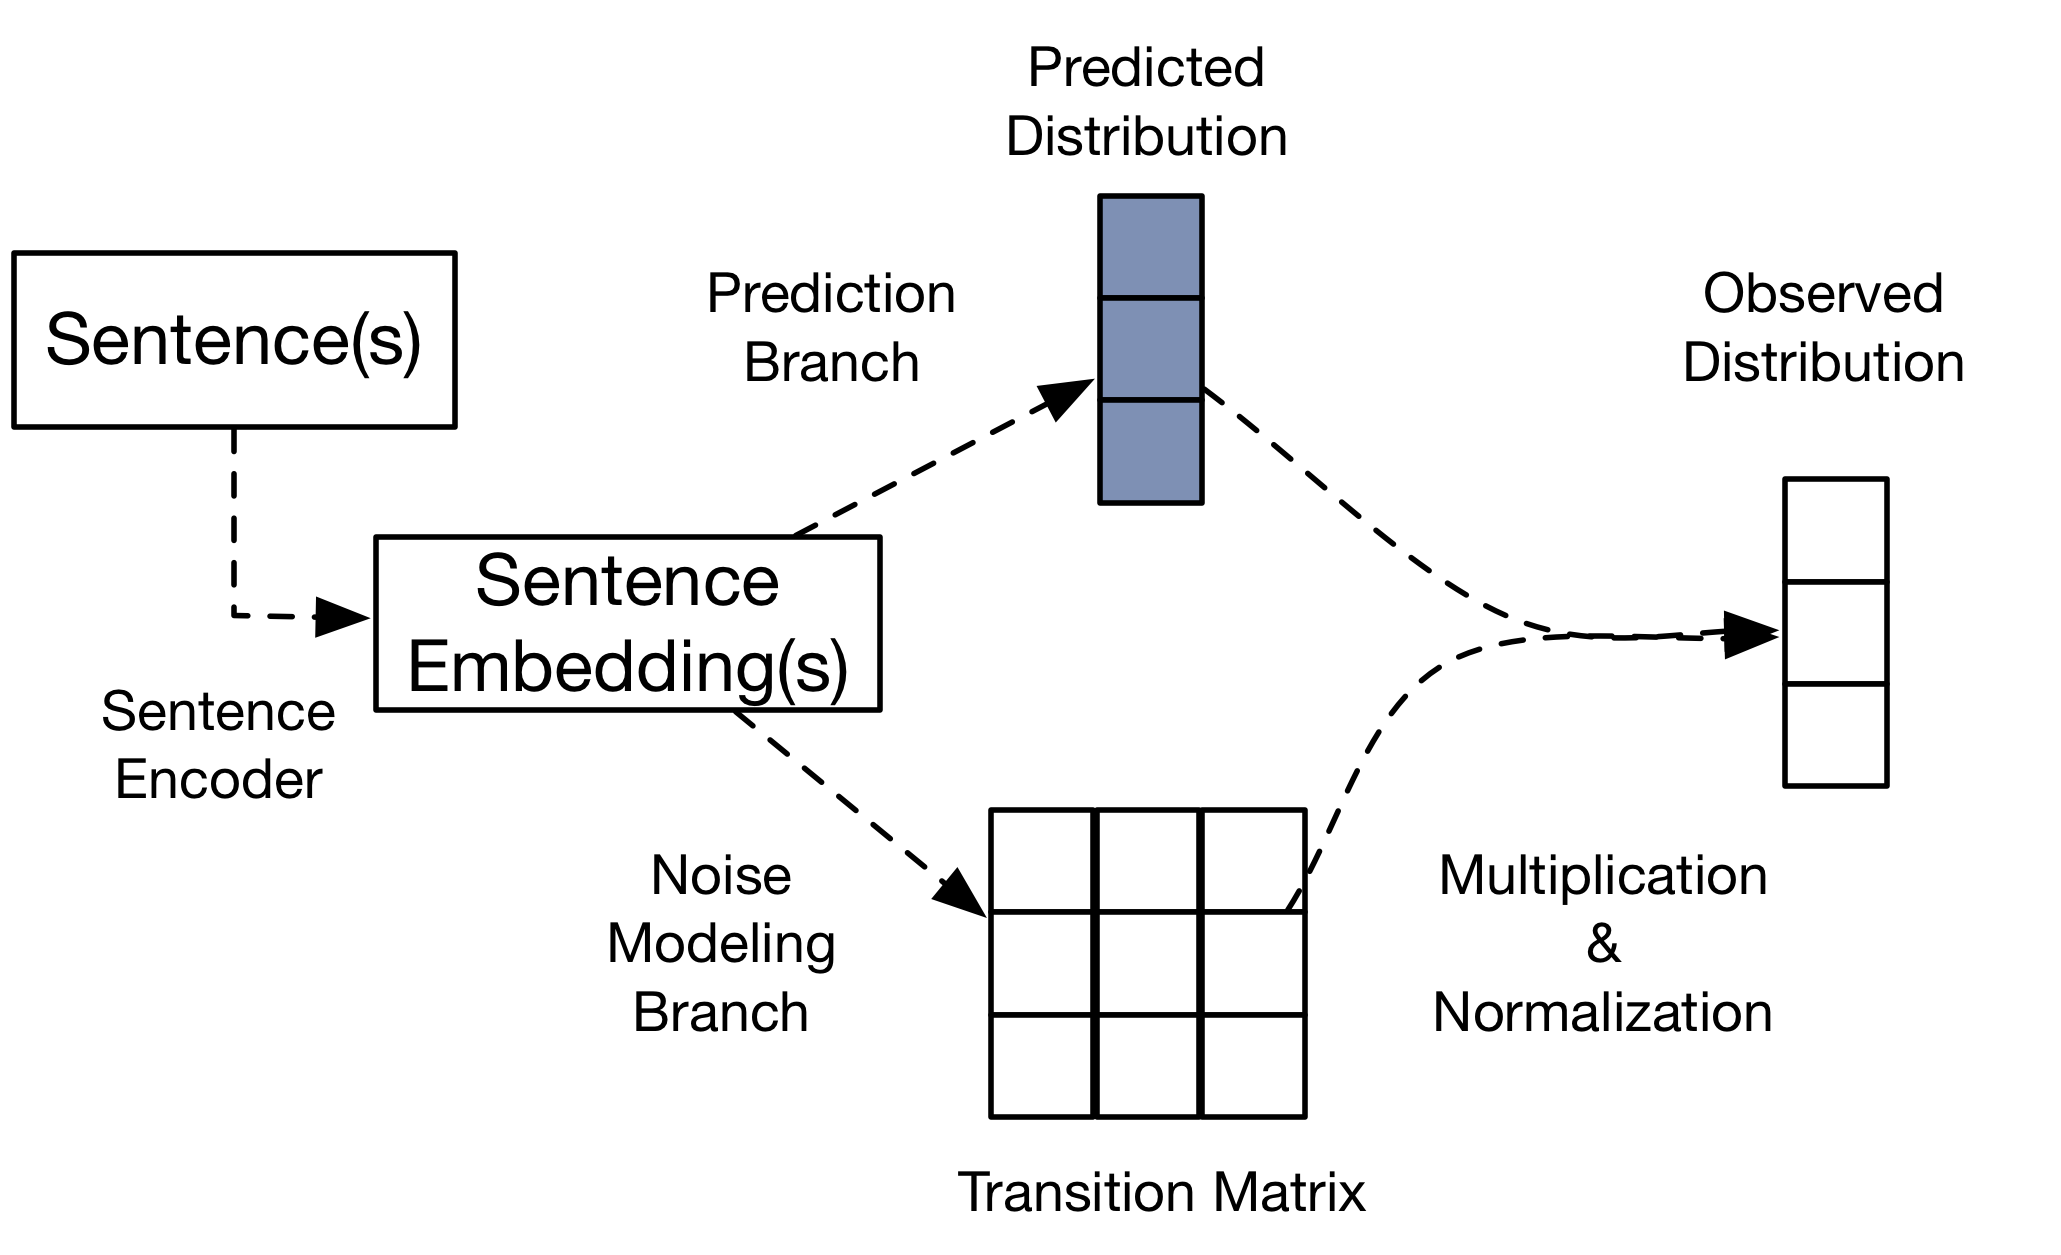
\includegraphics[width=8cm]{figures/denoise_framework.png}	
\caption{Overview of our approach}
\label{fig: denoise_framework}
\end{center}
\end{figure}


\section{Our Approach}
An overview of our approach of distantly supervised relation extraction is depicted in Figure \ref{fig: denoise_framework}. 
First, the input sentence (or sentence
bag) is passed to a sentence encoder to get sentence embedding(s). After that, the model is split into two branches.
The prediction branch generates the predicted relation distribution $\mathbf{p}$ of the input sentence (or sentence
bag). The noise modeling branch generates the transition matrix $\mathbf{T}$. Finally, the predicted distribution is
multiplied by the transition distribution to generate the observed relation distribution $\mathbf{o}$. The predicted
relation distribution $\mathbf{p}$ is the output of the model while the observed relation distribution $\mathbf{o}$ is
used to simulate the relation assigned by distant supervision. In this way, the noise is modeled by the transition
matrix and the real
prediction is protected from the influence of the noise. In rest of this section, we will first describe the sentence level model, and then extend the model to bag level.

\subsection{Sentence Encoder}
The sentence encoder serves to transform an input sentence to an embedding vector that encodes semantic meaning of the sentence. Theoretically, almost any sentence encoder would work here. Similar to previous researches, we also use the piecewise convolutional neural network (PCNN) model \cite{zeng2015distant} as our sentence encoder. First, the distances of each word to the subject and the object are embedded as randomly initialized vectors and concatenated to the original word vector. After that, the PCNN model divides the input sentence into three pieces by the subject and the object, and apply convolutional neural network (CNN) to each piece to calculate the piece embedding. The final sentence embedding is the concatenation of the embeddings of the three pieces.

\subsection{Prediction Branch}
The prediction branch generates the predicted relation distribution $\mathbf{p}$ and can be implemented by the prediction part of almost any relation extraction neural network models. Similar to \cite{luo2016temporal}, for sentence level models, we first feed the sentence embedding to a full connection layer, and then use softmax for relation classification.

\subsection{Noise Modeling Branch}
The noise modeling branch calculates a transition matrix dynamically for each sentence (or sentence bag) to model its noise pattern.

For sentence level models, the sentence embedding $\mathbf{x}$ is passed to another full connection layer to obtain the sentence embedding $\mathbf{x}_n$ used specifically for noise modeling branch. The transition matrix $\mathbf{T}$ is calculated using softmax function :
\begin{equation}
T_{ij} = \frac{exp({\mathbf{w}_{ij}^T \mathbf{x}_n + b})}{\sum_{j=1}^{|\mathbb{C}|}{exp({\mathbf{w}_{ij}^T \mathbf{x}_n + b}})}
\end{equation}
where $T_{ij}$ is the conditional probability that this sentence is labeled as relation $j$ by distant supervision given $i$ as the true relation, $\mathbf{w}_{ij}$ is the weight vector for this situation, $b$ is a scalar bias and $|\mathbb{C}|$ is the number of relations. Note that the softmax function guarantees that each row of the transition matrix $\mathbf{T}$ sums to 1.

\subsection{Observed Relation Distribution}
The observed relation distribution $\mathbf{o}$ is calculated by multiplying transition matrix $T$ and the predicted relation distribution $p$:
 \begin{equation}
\mathbf{o} = \mathbf{T}^T \bm\cdot \mathbf{p}
\label{eq_transition}
 \end{equation}
 \iffalse
 \begin{equation}
 \label{norm_o}
 o_i = \frac{o_i}{\sum_i{o_i}}
 \end{equation}
 \fi
 where $\bm\cdot$ represents dot product and we normalizes the elements of $\mathbf{o}$ so that $\sum_i{o_i}=1$ afterwards.

Different from previous works that use the predicted relation distribution $\mathbf{p}$ to directly match the relation labeled by distant supervision. \orange{We instead use $\mathbf{o}$ to match the noisy label and still use $\mathbf{p}$ as output}. Note that if the true relation of the input training instance is $i$, we can assume that this relation $i$ could be labeled as relation $j$ by distant supervision with probability $T_{ij}$. Therefore, Equation \ref{eq_transition} actually models the procedure of how the noisy label is produced and thus \orange{protects $\mathbf{p}$ from the bad influence of noise.}
%can help the model make better use of the noisy training data. \red{How to better use?? by using regularization????}

Also note that the noise modeling branch and $\mathbf{o}$ is only used in the training phase. In the test phase, we only use the prediction brach and take the predicted relation distribution $\mathbf{p}$ as our output. \todo{last paragraph can be removed}

\subsection{Bag Level Models}
\paragraph{Bag Level Prediction Branch}
The key problem in the bag level prediction branch is how to aggregate the embeddings of each sentence in the bag. Here we experiment with two methods, average and attention aggregation. The average aggregation calculates the bag embedding $\mathbf{s}$ by averaging the embeddings of each sentence, and the resultant bag embedding is fed to a softmax classifier for relation classification.

The attention aggregation method is proposed by \cite{lin2016neural}. It calculates an attention value for each sentence with respect to each relation, and uses the following equation to calculate the bag embedding with respect to relation $j$:
\begin{equation}
\mathbf{s}_j = \sum_i^{n}{\alpha_{ij} \mathbf{x}_{i}}
\label{eq_att_bag_embed}
\end{equation}
where $\mathbf{x}_{i}$ is the embedding of sentence $i$, $n$ is the number of sentences in the bag and $\alpha_{ij}$ is the attention value over sentence $i$ with respect to relation $j$. The resultant bag embedding is fed to a softmax classifier to predict the probability of relation $j$.

\paragraph{Bag Level Transition Matrix}
\orange{We use attention mechanism to generate transition matrix for both average and attention aggregation models.} Specifically, we calculate the bag embedding with respect to each relation with Equation \ref{eq_att_bag_embed}, and the attention value for sentence $i$ with respect to relation $j$ is calculated by:
\begin{equation}
\alpha_{ij} = \frac{exp(\mathbf{x}_i^T \mathbf{r}_t^j)}{\sum_i^n{exp(\mathbf{x}_i^T \mathbf{r}_t^j)}}
\end{equation}
where $\mathbf{x}_i$ is the embedding of sentence $i$ and $\mathbf{r}_t^j$ is the randomly initialized embedding of relation $j$ used specifically for noise modeling branch.

Then the transition matrix $\mathbf{T}$ is calculated by:
\begin{equation}
T_{ij} = \frac{exp({\mathbf{s}_i^T \mathbf{r}_t^j  + b})}{\sum_{j=1}^{|\mathbb{C}|}{exp(\mathbf{s}_i^T \mathbf{r}_t^j + b})}
\end{equation}
where $\mathbf{s}_i$ is the bag embedding with respect to relation $i$, $\mathbf{r}_t^j$ is the same embedding of relation $j$.


\section{Training Procedure}
\red{I would suggest to move some of the motivations to the Introduction part,  we need to motivate regularization and CL there.}The difficulty of training the transition matrix lies in that there is no direct guidance over the noise pattern. The only supervision we have is the noisy label produced by distant supervision. However, if we have prior knowledge to roughly separate the data into reliable and unreliable parts, we can use the split as indirect supervision over the noise pattern by letting the model treat these data differently. In this section, we describe how to use trace regularization to control the behavior of the transition matrix. Furthermore, instead of modeling the noise at the very beginning of the training, we emphasis noise modeling gradually by building different curriculums in the situation with and without prior knowledge of the data quality under the curriculum learning framework.
%Apart from that, we also show how to constrain the \red{ability??} of the transition matrix to avoid \red{overfitting???}.

\subsection{Trace Regularization}
Intuitively, if the noise is small, the transition matrix $\mathbf{T}$ will tend to become an identity matrix (vice versa).  Since each row of $\mathbf{T}$ sums to 1, the similarity between the transition matrix and the identity matrix can be represented by the trace of the transition matrix $\mathbf{T}$. The larger the $trace(\mathbf{T})$ is, the smaller the elements that do not lie in the diagonal are, and the more similar the transition matrix $\mathbf{T}$ is to identity matrix. Therefore, we can realize our expectation over the noise level of the data by controlling the value of $trace(\mathbf{T})$.

\subsection{Curriculum Learning}
The basic idea of curriculum learning is simple: start with the easiest aspect of a task, and level up the difficulty gradually.

\paragraph{With Prior Knowledge of Data Quality}
If we have prior knowledge about which part of the training data is more reliable and which is unreliable, the most straightforward way to build a curriculum is by controlling the reliability of training data. Specifically, we can first train the prediction branch on the reliable data for some epochs and then add the unreliable data \orange{to train the full model}. In this way, the prediction branch is roughly trained before exposed to more noisy data.

Furthermore, \orange{we can also take better control of the training procedure by trace regularization.}
%\red{utilize our prior knowledge of the data quality in the form of trace regularization}.
Specifically, our loss function is:

\begin{equation}
\begin{aligned}
Loss=\sum_{i=1}^M{\sum_{j=1}^{N_i}{-log(o_{ijy_{ij}})}} + \beta_i trace(\mathbf{T}_{ij})
\end{aligned}
\end{equation}
where the left side is vanilla cross entropy and the right side is trace regularization, $i$ is the index of the data subsets, $j$ is the index of training data, $\beta_i$ is the trace regularization weight for subset $i$, $\mathbf{T}_{ij}$, $y_{ij}$ and $o_{ijy_{ij}}$ are the transition matrix, relation labeled by distant supervision, and the observed probability of that relation for datum $j$ in subset $i$ respectively.

For the reliable subset, we want $trace(\mathbf{T})$ to be large (negative $\beta$) so that the element values of $\mathbf{T}$ will be centralized to the diagonal and the transition matrix will be similar to identity matrix. As for the unreliable subsets, we want the $trace(\mathbf{T})$ to be small (positive $\beta$) so that the element values of their transition matrices will be diffusive \orange{and the transition matrix will be less similar to identity matrix. In other words, the transition matrix is encouraged to model the noise}. Note that this loss function only works for sentence level models, since reliable sentences and unreliable ones are all aggregated into a sentence bag in the bag level models and therefore we can not determine which bag is reliable and which is not. However, bag level models can still use the curriculum by changing the content of the bag, \orange{and can therefore benefit from the prior knowledge of data quality.}

\paragraph{Without Prior Knowledge of Data Quality}
\label{curr_over_data}
If we do not have prior knowledge about the quality of training data, we can still build a curriculum, which can be used in all situations, \orange{by controlling the training objective to gradually emphasis on noise modeling. Specifically, we design a decreasing weighting scheme for both the cross entropy of output prediction and the trace regularization component: (CHANGE EXPLAINATION: the decreasing scheme is for both $\alpha$ and $\beta$, not just $\beta$.)}
%\red{ gradually controlling the impact of the transition matrix}. Specifically, \red{we design a decreasing weighting scheme for the trace regularization component}, defined as:

\begin{equation}
\begin{aligned}
Loss	&=\sum_{i=1}^N{-((1-\alpha) log(o_{iy_{i}}) + \alpha log(p_{iy_{i}}))} \\
&+ \beta trace(\mathbf{T}_{i})
\end{aligned}
\end{equation}
where $0\le\alpha\le1$, $y_i$ is the relation assigned by distant supervision for datum $i$, $o_{iy_{i}}$ and $p_{iy_{i}}$ are the probabilities that the observed and predicted relation for datum $i$ is $y_i$ respectively. Instead of only using the observed relation distribution $\mathbf{o}$ to simulate the relation labeled by distant supervision, we use the linear combination of the cross entropy of both the observed relation distribution $\mathbf{o}$ and the predicted relation distribution $\mathbf{p}$.

\orange{We consider ignoring the noise is easier than modeling the noise. Therefore, to build a curriculum}, we set $\alpha=1$ and $\beta<0$ at the start of the training, which means we do not expect to model the noise. As the training proceeds, the prediction branch gradually learns the basic prediction ability, then we increase the difficulty level by decreasing $\alpha$ and the absolute value of $\beta$ by $\rho$ every $\tau$ epochs to gradually guide our model to learn to model the noise.

\subsection{Constrained Transition Matrix}
\orange{Since the triples in knowledge base are reliable in most of the times, the positive label confusion noise is less likely than the false negative and false positive noise.} However our transition matrix has the ability to model all these three types of noise. To prevent overfitting and make the model \red{concentrate on the false negative and false positive noise??}\orange{(not sure about the problem)}, we restrict the transition matrix for bag level models so that only the diagonal, the first column and the first row of the transition matrix do not equal to zero (assume the index of \emph{no-relation} is 0).
